% % % % % % % % % % % % % % % % % % % % % % % % % % % % % % % % % % % % %
% Chapter: Experiment 1
% % % % % % % % % % % % % % % % % % % % % % % % % % % % % % % % % % % % %
\chapter{Experiment 1: Using random input}
\label{cpt:experiment1}
\pinfo{Props to test cases, implication returns True}
The properties that we defined in \autoref{cpt:properties} are translated into
test cases as described in \autoref{cpt:testmechanics}. In this experiment we
expect to find some bugs that were unknown before by using the test framework.
When we have triggered some bugs, an investigation is needed to check what the
cause is of that bug. Next, we can categorize the bugs found to come to an
answer to this research question:\rqThree{}

% % % % % % % % % % % % % % % % % % % % % % % % % % % % % % % % % % % % %
% Section: Method
\section{Method}
%\label{sec:initial_case}
\pinfo{Like QuickCheck, recall cycle shortly}
In the first experiment each property will be tested 100 times with random input
values. This means that if the property holds for 100 tests, it is reported to be successfully satisfying the property. This is a similar approach as what \textit{QuickCheck} does when
checking properties. Unlike \textit{QuickCheck}, the test framework does not shrink the input values to come with minimum values for which the case fails. Instead it will just report the values that were used when the property failed.

% % % % % % % % % % % % % % % % % % % % % % % % % % % % % % % % % % % % %
% Section: Results
\section{Results}
In this experiment two runs are being done to detect bugs in the generator. The
first run terminated quickly, which is why the test framework did not succeed in
testing every property.

% % % % % % % % % % % % %
% Subsection: First run
\subsection{First run}
\pinfo{Termination, compile error due to library}
The first run results into a termination of the run due to a compile error in the generated system. Although we made the assumption that the generated system should be compilable, this error came from a property definition that was expected to hold, namely \textit{AssociativeMultiplicationInteger1} (\autoref{ssct:4_associativity}). Which is why we can consider this as an error that is found when using the test framework. The error describes that an overloaded method cannot be applied to the \textit{Money} type, as shown in \autoref{lst:ch5_firstrun_termination_log}.
% Listing
\FloatBarrier
\begin{sourcecode}[!ht]
\begin{lstlisting}[language=Log]
[error] MoneySpec.scala:316: overloaded method value * with alternatives:
[error]   (x: Double)Double <and>
[error]   (x: Float)Float <and>
[error]   (x: Long)Long <and>
[error]   (x: Int)Int <and>
[error]   (x: Char)Int <and>
[error]   (x: Short)Int <and>
[error]   (x: Byte)Int
[error]  cannot be applied to (squants.market.Money)
[error]           Initialised(Data(result = Some(((((x * y)) * z) == (x * ((y * z)))))))
[error]                                                                 ^
[error] MoneySpec.scala:441: overloaded method value * with alternatives:
[error]   (x: Double)Double <and>
[error]   (x: Float)Float <and>
[error]   (x: Long)Long <and>
[error]   (x: Int)Int <and>
[error]   (x: Char)Int <and>
[error]   (x: Short)Int <and>
[error]   (x: Byte)Int
[error]  cannot be applied to (squants.market.Money)
[error]             checkPostCondition((nextData.get.result.get == (((((x * y)) * z) == (x * ((y * z)))))), "new this.result == ( (x*y)*z == x*(y*z) )")
[error]                                                                                    ^
[error] two errors found
[error] (compile:compileIncremental) Compilation failed
[error] Total time: 79 s, completed 4-aug-2017 13:03:45
> Done testing
> ** Some tests failed! **
\end{lstlisting}
\caption{Log output first test run resulting in a termination.}
\label{lst:ch5_firstrun_termination_log}
\end{sourcecode}
\todo{Up arrow is incorrectly aligned in the listing due to layout}
\FloatBarrier
% End listing
\pinfo{Investigation, found property and var types}
The error log does not clearly indicate what is exactly going wrong, it doesn't show which property is causing it, also it does not describe what the types of the variables were. Investigating the generated system reveals that both errors were happening when dealing with the \textit{AssociativeMultiplicationInteger1} property. This means that the variables x, y and z are of type \textit{Integer}, \textit{Integer}, \textit{Money} respectively, as described in \autoref{ssct:4_associativity}. Temporarily disabling this property allows the test framework to proceed further.

% % % % % % % % % % % % %
% Subsection: Second run
\subsection{Second run}
\pinfo{Failing tests, describing each}
After disabling the \textit{AssociativeMultiplicationInteger1} property, the test framework was able to run completely. This results in 7 failing tests. For each test the input values for which the property doesn't hold are logged such that the error can be reproduced. In \autoref{tbl:experiment1_overview_second_run} an overview of the failing properties, along with it's input values (\textit{x}, \textit{y} and \textit{z}) are shown.
% Table
\FloatBarrier
\begin{table}[!ht]
\centering
\begin{tabular}{llll}
\hline
\textbf{Property name}               & \textbf{x}               & \textbf{y}        & \textbf{z}         \\ \hline
DistributivePercentage1              & 0.51                     & -311254801.77 EUR & -707194075.77 EUR  \\
DistributivePercentage2              & 0.93                     & 2089630160.75 EUR & -1316628389.49 EUR \\
DistributiveInt2                     & -883022216               & -298435082.93 EUR & 715725888.96 EUR   \\
AssociativeMultiplicationPercentage2 & 840296462                & 1771903729.60 EUR & 0.53               \\
DistributiveInt1                     & -1790274467.41 EUR       & 1691684272        & 1449321647         \\
AssociativeMultiplicationInteger2    & -1852801029.34 EUR       & -1309504561       & 1880170895         \\
AssociativeMultiplicationPercentage1 & -352883323.42 EUR        & 0.27              & 294211708          \\ \hline
\end{tabular}
\caption{Overview of failing tests along with its input values}
\label{tbl:experiment1_overview_second_run}
\end{table}
\FloatBarrier
% End table


% % % % % % % % % % % % % % % % % % % % % % % % % % % % % % % % % % % % %
% Section: Analysis
\section{Analysis}
For each failed test we investigate what went wrong. The first four tests reveal precision problems when using the \textit{Money} type in calculations. The latter three tests were also failing because of these precision problems. However, these tests were also failing after the precision errors were fixed. Thus, for the latter 3 tests another version of the generated system was used, which contains the fixes for the precision problems. This is done such that we are able to reveal the other errors that these properties can reveal.

\todo{Add red in tables}
% % %
% Explaining failing cases.
% % %
% % %
% DistributivePercentage1
\subsubsection{DistributivePercentage1}
\label{ssct:ch5_distributivePercentage1}
This property uses a \textit{Percentage} value and two \textit{Money} values for its tests. The values are named x, y and z respectively. To check this failing test, we check the results of the intermediate calculations in the formula that is being used. In \autoref{ch4_init_check_DistributivePercentage1} values are shown for which the test case fails, among with the intermediate calculations. The intermediate calculations seem to work as expected, as the results are the same when we compare the results of the Scala evaluation and the Rascal evaluation. Unfortunately the resulting left hand side of the expression contains a precision error, which is caused when multiplying a \textit{Percentage} (the x variable) with a \textit{Money} type (the result of y+z in this case).
% Table
\FloatBarrier
\begin{table}[!ht]
\centering
\begin{tabular}{rll}
\hline
\textbf{Variable}      & \textbf{Value}          & \textbf{Type}            \\ \hline
X                      & 0.51                    & Percentage               \\
Y                      & -311254801.77 EUR       & Money                    \\
Z                      & -707194075.77 EUR       & Money                    \\ \hline
\textbf{Formula}       & \textbf{Scala result}   & \textbf{Expected result} \\ \hline
x*(y+z) == (y*x)+(z*x) & false                   & true                     \\
x*(y+z)                & -519408927.54539996 EUR & -519408927.5454 EUR      \\
(y*x)+(z*x)            & -519408927.5454 EUR     & -519408927.5454 EUR      \\
                       &                         &                          \\
y+z                    & -1018448877.54 EUR      & -1018448877.54 EUR       \\
y*x                    & -158739948.9027 EUR     & -158739948.9027 EUR      \\
z*x                    & -360668978.6427 EUR     & -360668978.6427 EUR      \\ \hline
\end{tabular}
\caption{DistributivePercentage1: Precision error when multiplying a \textit{Percentage} with \textit{Money}}
\label{ch4_init_check_DistributivePercentage1}
\end{table}
\FloatBarrier
% End table

% % %
% DistributivePercentage2
\subsubsection{DistributivePercentage2}
This test case looks similar than the \textit{DistributivePercentage1} (\autoref{ssct:ch5_distributivePercentage1}). It uses the same type of variables, but the expression is slightly different. In \autoref{ch4_init_check_DistributivePercentage2} the result and the intermediate calculations of a failing case are shown. What can be seen here is that the precision error occurs when the Money type is multiplied by the Percentage type. While in \autoref{ssct:ch5_distributivePercentage1} it was the other way around.
% Table
\FloatBarrier
\begin{table}[!ht]
\centering
\begin{tabular}{rll}
\hline
\textbf{Variable}      & \textbf{Value}          & \textbf{Type}            \\ \hline
X                      & 0.93                    & Percentage               \\
Y                      & 2089630160.75 EUR       & Money                    \\
Z                      & -1316628389.49 EUR      & Money                    \\ \hline
\textbf{Formula}       & \textbf{Scala result}   & \textbf{Expected result} \\ \hline
(y+z)*x == (y*x)+(z*x) & false                   & true                     \\
(y+z)*x                & 718891647.2718 EUR      & 718891647.2718 EUR       \\
(y*x)+(z*x)            & 718891647.2718001 EUR   & 718891647.2718 EUR       \\
                       &                         &                          \\
y+z                    & 773001771.26 EUR        & 773001771.26 EUR         \\
y*x                    & 1943356049.4975002 EUR  & 1943356049.4975 EUR      \\
z*x                    & -1224464402.2257001 EUR & -1224464402.2257 EUR     \\ \hline
\end{tabular}
\caption{DistributivePercentage1: Precision error when multiplying a \textit{Money} with \textit{Percentage}}
\label{ch4_init_check_DistributivePercentage2}
\end{table}
\FloatBarrier
% End table

% % %
% DistributiveInt2
\subsubsection{DistributiveInt2}
\label{ssct:ch5_distributiveInt2}
This case uses \textit{Integer} in conjunction with the \textit{Money} type. Earlier cases showed that there was a precision error when using the \textit{Percentage} and \textit{Money} types. Since the \textit{Percentage} type is translated to a \textit{Double} in the generated system, it can be expected that there would be precision problems occuring. As this is a known issue with types that use floating-point arithmetic \cite{goldberg1991every}. This case reveals that a precision error also occurs when multiplying \textit{Money} with an \textit{Integer}. In the intermediate calculations when investigating a failing test with it's values are shown in \autoref{ch4_init_check_DistributiveInt2}. The last two rows, colored in red, show that a precision error occurs when \textit{Money} is multiplied by an \textit{Integer}.
% Table
\FloatBarrier
\begin{table}[!ht]
\centering
\begin{tabular}{rll}
\hline
\textbf{Variable}  & \textbf{Value}          & \textbf{Type}              \\ \hline
X                  & -883022216              & Integer                    \\
Y                  & -298435082.93 EUR       & Money                      \\
Z                  & 715725888.96 EUR        & Money                      \\ \hline
\textbf{Formula}   & \textbf{Scala result}   & \textbf{Expected result}   \\ \hline
(x*y)*z == x*(y*z) & false                   & true                       \\
(x*y)*z            & -368477052257036740 EUR & -368477052257036762.48 EUR \\
x*(y*z)            & -368477052257036796 EUR & -368477052257036762.48 EUR \\
                   &                         &                            \\
y+z                & 417290806.03 EUR        & 417290806.03 EUR           \\
y*x                & 263524808260992384 EUR  & 263524808260992372.88 EUR  \\
z*x                & -632001860518029180 EUR & -632001860518029135.36 EUR \\ \hline
\end{tabular}
\caption{DistributiveInt2: Precision error when multiplying Money with an Integer}
\label{ch4_init_check_DistributiveInt2}
\end{table}
\FloatBarrier
% End table

% % %
% AssociativeMultiplicationPercentage2
\subsubsection{AssociativeMultiplicationPercentage2}
The earlier cases already shown a precision error when using Doubles and Integers in conjunction with \textit{Money}. This case triggers the same problem, but also reveals that the same thing happens when multiplying an \textit{Integer} with \textit{Money}. While in \autoref{ssct:ch5_distributiveInt2} it was the other way around. The intermediate calculations are shown in \autoref{ch4_init_check_AssociativeMultiplicationPercentage2}, the calculation of multiplying an Integer with Money is shown in red. Additionally, this case shows that the small precision error that we've seen earlier can cause a seemingly difference, which is a difference of 130 EUR in this case.
% Table
\FloatBarrier
\begin{table}[!ht]
\centering
\begin{tabular}{rll}
\hline
\textbf{Variable}  & \textbf{Value}          & \textbf{Type}              \\ \hline
X                  & 840296462               & Integer                    \\
Y                  & 1771903729.60 EUR       & Money                      \\
Z                  & 0.53                    & Percentage                 \\ \hline
\textbf{Formula}   & \textbf{Scala result}   & \textbf{Expected result}   \\ \hline
(x*y)*z == x*(y*z) & false                   & true                       \\
(x*y)*z            & 789129950543366910 EUR  & 789129950543366877.856 EUR \\
x*(y*z)            & 789129950543366780 EUR  & 789129950543366877.856 EUR \\
                   &                         &                            \\
x*y                & 1488924434987484670 EUR & 1488924434987484675.2 EUR  \\
y*z                & 939108976.688 EUR       & 939108976.688 EUR          \\ \hline
\end{tabular}
\caption{AssociativeMultiplicationPercentage2: Precision error causing bigger differences}
\label{ch4_init_check_AssociativeMultiplicationPercentage2}
\end{table}
\FloatBarrier
% End table

% % %
% DistributiveInt1
\subsubsection{DistributiveInt1}
This case also uses three variables: x, y and z. Which are of type \textit{Money}, \textit{Integer} and \textit{Integer} respectively. In \autoref{ch4_init_check_DistributiveInteger1} the different values are shown of the calculation between Scala and the expected result. The red line shows how the addition of two (positive) Integers results in a negative value. The result value would be bigger than the maximum value of an \textit{Integer}, causing it to overflow. Thus the operation also does not check or prevent against overflowing. \todo{SOURCE-Over/underflow}
% Table
\FloatBarrier
\begin{table}[!ht]
\centering
\begin{tabular}{rll}
\hline
\textbf{Variable}      & \textbf{Value}              & \textbf{Type}               \\ \hline
X                      & -1790274467.41 EUR          & Money                       \\
Y                      & 1691684272                  & Integer                     \\
Z                      & 1449321647                  & Integer                     \\ \hline
\textbf{Formula}       & \textbf{Scala result}       & \textbf{Expected result}    \\ \hline
x*(y+z) == (x*y)+(x*z) & false                       & true                        \\
x*(y+z)                & 2065907589620385223.57 EUR  & -5623262698769382599.79 EUR \\
(x*y)+(x*z)            & -5623262698769382599.79 EUR & -5623262698769382599.79 EUR \\
                       &                             &                             \\
y+z                    & -1153961377                 & 3141005919                  \\
x*y                    & -3028579159080673575.52 EUR & -3028579159080673575.52 EUR \\
x*z                    & -2594683539688709024.27 EUR & -2594683539688709024.27 EUR \\ \hline
\end{tabular}
\caption{DistributiveInteger1: \textit{Integer} overflows when using addition}
\label{ch4_init_check_DistributiveInteger1}
\end{table}
\FloatBarrier
% End table

% % %
% AssociativeMultiplicationInt2
\subsubsection{AssociativeMultiplicationInteger2}
% - Integer overflows, causing negative values etc.
For this case three variables are used: x, y and z, which are of type \textit{Money}, \textit{Integer} and \textit{Integer} respectively. In \autoref{ch4_init_check_AssociativeMultiplicationInteger2} the values of a failing test case are shown with the intermediate formula steps. On the left side of the expression we see the expected results, while on the right side there is a big difference. The red colored row shows a huge difference in the resulting values between Scala and the expected value of the intermediate step on this expression. The result value of the operation is smaller than the minimum value of an \textit{Integer}. Causing it to underflow, resulting in an unexpected amount as result. Thus the operation neither checks for underflowing an \textit{Integer} value, nor does it prevent it.\todo{SOURCE-Over/underflow}
% Table
\FloatBarrier
\begin{table}[!ht]
\centering
\begin{tabular}{rll}
\hline
\textbf{Variable}  & \textbf{Value}                      & \textbf{Type}                       \\ \hline
X                  & -1852801029.34 EUR                  & Money                               \\
Y                  & -1309504561                         & Integer                             \\
Z                  & 1880170895                          & Integer                             \\ \hline
\textbf{Formula}   & \textbf{Scala result}               & \textbf{Expected result}            \\ \hline
(x*y)*z == x*(y*z) & false                               & true                                \\
(x*y)*z            & 4561767263499657218201769467.30 EUR & 4561767263499657218201769467.30 EUR \\
x*(y*z)            & 3877739486117270379.94 EUR          & 4561767263499657218201769467.30 EUR \\
                   &                                     &                                     \\
x*y                & 2426251398546224819.74 EUR          & 2426251398546224819.74 EUR          \\
y*z                & -2092906591                         & -2462092362461952095                \\ \hline
\end{tabular}
\caption{AssociativeMultiplicationInteger2: \textit{Integer} underflows when using multiply}
\label{ch4_init_check_AssociativeMultiplicationInteger2}
\end{table}
\FloatBarrier
% End table

% % %
% AssociativeMultiplicationPercentage1
\subsubsection{AssociativeMultiplicationPercentage1}
% - Generating big double, precision can't be known for Squants!
In this case there are three variables: x, y and z, which are of type
\textit{Money}, \textit{Percentage} and \textit{Integer} respectively. In Table
\ref{ch4_init_check_AssociativeMultiplicationPercentage1} the values and
intermediate calculations are shown of a failing case, such that we can reason
about the results. The row marked in red shows a precision error when comparing
the results of Scala and Rascal with each other. This issue is caused by the
\textit{Percentage} that is being used. In the implementation, the
\textit{Percentage} is actually being translated into a \textit{Double}, which
is being multiplied with an \textit{Integer}. This results in a \textit{Double}
value containing a precision error, which is related to the problems with
floating-point arithmetic \cite{goldberg1991every}.
% Table
\FloatBarrier
\begin{table}[!ht]
\centering
\begin{tabular}{rll}
\hline
\textbf{Variable}  & \textbf{Value}         & \textbf{Type}               \\ \hline
X                  & -352883323.42 EUR      & Money                       \\
Y                  & 0.27                   & Percentage                  \\
Z                  & 294211708              & Integer                     \\ \hline
\textbf{Formula}   & \textbf{Scala result}  & \textbf{Expected result}    \\ \hline
(x*y)*z == x*(y*z) & false                  & true                        \\
(x*y)*z            & -28032049433190944 EUR & -28032049433190942.3672 EUR \\
x*(y*z)            & -28032049433190948 EUR & -28032049433190942.3672 EUR \\
                   &                        &                             \\
x*y                & -95278497.3234 EUR     & -95278497.3234 EUR          \\
y*z                & 79437161.16000001      & 79437161.16                 \\ \hline
\end{tabular}
\caption{AssociativeMultiplicationPercentage1: A precision error when using \textit{Percentage}}
\label{ch4_init_check_AssociativeMultiplicationPercentage1}
\end{table}
\FloatBarrier
% End table
Additionally, we can see a difference in the results on the left and right side of the expression evaluation in Scala. Where as the intermediate step for the left side is calculated correctly. This also hints to the bug in the \textit{Money} type which we already found with the `DistributiveInt2` test. For the right side we cannot say this immediately, as there is already an error in the intermediate step.\\
\\
This property revealed a precision error when the \textit{Percentage} type is being used. The \textit{Percentage} is being translated to a \textit{Double} value, causing operations with it to have precision errors. In this case the \textit{Percentage} is being multiplied by an \textit{Integer}.

% % % % % % % % % % % % % % % % % % % % % % % % % % % % % % % % % % % % %
% Section: Evaluation criteria
\section{Evaluation criteria}

% Property coverage
\pinfo{Not tested implicative properties}
When looking at the coverage results of the test suite, it is notable that the condition for the if-clause of the implicative properties are often not being triggered.  Resulting in that it always returns \textit{true}, as this is how it was specified in the specification (the else-clause of an implicative property). This is due to the random values that are being used as input. An example of this is the \textit{TransitiveEquality} property (\code{x == y \&\& y == z $\implies$ x == z}). When relying on random data, there is a seldom chance that 3 values are equal to each other. Thus we could optimize the random values such that the condition holds, such that we also test these properties such that the if-clause is triggered. In \autoref{fig:experiment1_coverage_implicative_property} the coverage for the \textit{TransitiveEquality} property, green highlighting indicate the statements that are executed, while red highlighting indicate statements that were not checked at all.
% Figure
\FloatBarrier
\begin{figure}[!ht]
%\frame{
	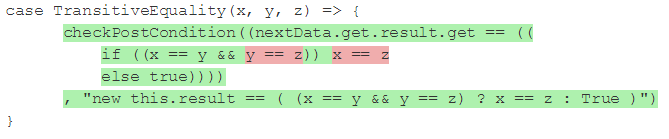
\includegraphics[width=\linewidth]{figures/experiment1_coverage_implicative_property}
%}
\caption{Test coverage of an implicative property (\textit{TransitiveEquality})}
\label{fig:experiment1_coverage_implicative_property}
\centering
\end{figure}
\FloatBarrier
% End figure

% Total coverage
\pinfo{Test coverage, 30\% for implicative, 100\% for others}
The first criteria to evaluate an experiment was to determine the test coverage. The properties using implication are not covered when using random values as input data. The other properties, which do not use implication, are fully tested though. This can be seen in \autoref{fig:experiment1_evaluation_result}, where the test coverage of the properties using implication only covers roughly 30\%. The files with a name ending with "Logic" contain the implementation of the properties, as well as the precondition checks. The test coverage concerning the other properties (those that do not use implication), reports 95\% coverage. When investigating further, the other 5\% are not related to the properties that we test, thus it is not required for this project to achieve 100\% coverage on the Logic files.
% Figure
\FloatBarrier
\begin{figure}[!ht]
%\frame{
	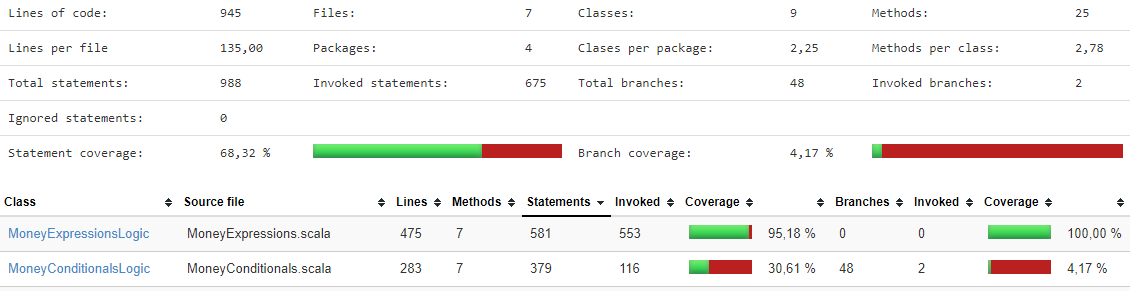
\includegraphics[width=\linewidth]{figures/eval_experiment1}
%}
\caption{Test coverage report of the first experiment}
\label{fig:experiment1_evaluation_result}
\centering
\end{figure}
\FloatBarrier
% End figure
\pinfo{Overall 68\%, cannot be 100, but can be improved}
The overall coverage over the generated system is 68\%. Note that the libraries that are being used by the generated system are not included in the coverage report. We expect that this number can be improved by generating values such that the properties using implication are also triggering the if-clause. Which is currently not the case, as we have seen when checking the coverage of an implicative property in \autoref{fig:experiment1_coverage_implicative_property}.\\
\\
% % of bugs
\pinfo{\# of bugs, 7}
The second criteria that we defined was the amount of bugs that we have found by doing the experiment. By using this approach we found a total of 4 bugs. A compilation error, overflow/underflow error and precision errors. 2 of these 4 bugs were related to the precision problem when using doubles, but one originated from the library that is used for the Money type, while the other is because the \textit{Percentage} type is translated to a \textit{Double}. Which is why we define these as 2 separate bugs. An improvement of the test suite to also cover the properties using implication might result in more bugs that can be found.

% % % % % % % % % % % % % % % % % % % % % % % % % % % % % % % % % % % % %
% Section: Conclusion
\section{Conclusion}
% 1: Squants using doubles internally. Small precision error can lead to bigger (unexpected) amounts as we've seen in AMP2.
% 	 - DistributivePercentage1: Multiplying Double with Money causes a precision error
%	 - DistributivePercentage2: Multiplying Money with Double causes a precision error
% 	 - DistributiveInt2: Multiplying Money with Integer
%    - AssociativeMultiplicationPercentage2: Multiplying Integer with Money. And with double. Causing big numbers to be losing precision anyway. Bug in Squants is the problem here though.
% 2: Operations on an Integer are over/underflowing, causing incorrect results.
%	 - AssociativeMultiplicationInt2: When using Multiply on Ints
%	 - DistributiveInt1: When using Addition on Ints
% 3: Percentage is double, causing big values to lose precision, which can cascade through the expressions
%	 - AssociativeMultiplicationPercentage1: Multiplying Percentage with Int, causing a big Double value with precision loss. Squants cannot guess the actual number anymore
\pinfo{Recap, found 7 bugs using this approach}
In this first experiment we tested each property that was defined in \autoref{cpt:properties} 100 times with using random values as input. First the test suit terminated due to a compilation error. After disabling the causing property (temporarily), a total of 7 tests were failing. In this experiment we managed to find precision errors and overflow/underflow errors. Additionally, we found a compilation error when using a property which was expected to hold.\\
\\
\pinfo{Implicative properties not tested}
Although many properties were tested succesfully, the test framework also indicates that the implicative properties were satisfied. However, when looking at the statement coverage of the implicative properties, we saw that the if-clause is often not being. Meaning that it would call the else-clause which simply returns true. When relying on random data, there is a seldom chance that the if-clause is being triggered. Thus we could optimize the generated input values such that these satisfy the condition for the if-clause.

% % % % % % % % % % % % % % % % % % % % % % % % % % % % % % % % % % % % %
% Section: Threats to validity
\section{Threats to validity}

\subsection*{Fixed amount of tries}
\pinfo{Fixed amount of tries not substantiated}
The 100 tries to check a property is a fixed number that is being used. But why exactly this number and not a higher or lower number? It might be the case that some errors are not triggered because of this fixed amount. Running more cases might be revealing an additional error, or it might not. In case it doesn't, it means that the test suite just requires more time to run the whole test suite, while it does not have an effect on the results. 100 seems to be an amount that works such that it consistently reports the same amount of failing tests, however this has checked by running it the test runs multiple times, also with using numbers like 300 or 50 for the amount. Also \textit{QuickCheck} uses this amount to check a property. During this thesis we stick with 100 as amount. Finding the optimal amount of tries is left as future work, thus remaining as a threat of validity in this approach.

\subsection*{Unfixed issue}
\pinfo{Compile error not fixed}
Unfortunately the compilation error has not been fixed throughout this project, however, it is an open issue on \textit{Github}. Some precision errors originated from a library used in the generated system, called Squants. An issue was created covering these precision errors, which were fixed in the next release of that library. As for the overflow and underflow errors, these occurred when using the \textit{Integer} type in \textit{Rebel}. When using the \textit{Integer} type, this might have been expected behaviour which causes this to happen. However, the generated system does not check whether this happens, nor does it prevent this. Additionally, we can consider this behaviour unexpected on the Integer type in
\textit{Rebel}, as \textit{Rebel} does not support any other kind of number type that can hold a bigger value. For example, compared to
Java, a \textit{BigDecimal} would be possible. We consider the overflow and underflow errors as unexpected, as the \textit{Rebel} language does not support other numeric types to hold a bigger value than an \textit{Integer} supports.
